\documentclass{beamer}
 
\usepackage[utf8]{inputenc}
\usepackage[english]{babel}
\usepackage{amsmath}
\usepackage{amsfonts}
\usepackage{amssymb}
\usepackage{graphicx} 
\usepackage{latexsym} 
\usepackage{listings}
\usepackage{xcolor}
\usepackage{soul}
\usepackage[T1]{fontenc}
\usepackage{amsthm}
\usepackage{mathtools}
\usepackage{setspace}
\usepackage{array,multirow,makecell}
\usepackage{geometry}
\usepackage{textcomp}
\usepackage{float}
\usepackage{bbold}
\usepackage{wrapfig}
\usepackage{textpos}

\rmfamily

\usetheme{Madrid}
%%\usecolortheme{beaver}



\title{LP 14 Machines thermiques réelles}
\author{Naïmo Davier}
\institute{Université Paul sabatier}

 
\begin{document}
	
\begin{frame}
	\titlepage
\end{frame}

\addtocounter{framenumber}{-1}
\title{Machines thermiques réelles}

\begin{frame}
\frametitle{Diagramme de Raveau}
\centerline{\includegraphics[width=8.5cm]{raveau}}
\end{frame}

\begin{frame}
\frametitle{Cycle de Carnot}
\centerline{\includegraphics[width=12cm]{cycle_carnot}}
\end{frame}

\begin{frame}
\frametitle{Moteur à explosion}
\centerline {\includegraphics[width=6.5cm]{moteur_4_temps}
			\includegraphics[width=6cm]{cycle_explosion} }
\centerline {\includegraphics[width=6cm]{vilebrequin}}
\end{frame}

\begin{frame}
\frametitle{Cycle de Beau de Rochas}
\centerline{\includegraphics[width=8cm]{cycle_beau_de_rochas}}
\end{frame}

\begin{frame}
\frametitle{Cycle diesel}
\centerline {\includegraphics[width=8cm]{cycle_diesel}}
\end{frame}


\begin{frame}
\frametitle{Calcul du rendement pour le cycle diesel}
\begin{eqnarray}
Q_1 =  mC_p(T_C-T_B) \hspace{0.4cm}\mathrm{et} \hspace{0.4cm} Q_2 =  mC_v(T_A-T_D)\\
\eta = 1 + \frac{Q_1}{Q_2} = 1 + \frac{C_v}{C_p}\frac{T_A-T_D}{T_C-T_B} = 1+ \gamma^{-1}\frac{T_A-T_D}{T_C-T_B}
\end{eqnarray}
On a deux adiabatiques réversibles
\begin{eqnarray}
\frac{T_A}{T_B} = \left(\frac{V_A}{V_B}\right)^{1-\gamma} = a^{1-\gamma}\hspace{0.4cm}\mathrm{et} \hspace{0.4cm}  \frac{T_D}{T_C} = \left(\frac{V_D}{V_C}\right)^{1-\gamma} = b^{1-\gamma}
\end{eqnarray}
et une isobare : $\frac{V}{T} = $ cste
\begin{eqnarray}
\frac{V_C}{T_C} = \frac{V_B}{T_B} \Rightarrow \frac{T_B}{T_C} = \frac{V_B}{V_C} = \frac{b}{a}\;\; \mathrm{puisque}\;\; V_D=V_A
\end{eqnarray}
on obtient alors finalement
\begin{eqnarray}
\rightarrow \frac{T_A-T_D}{T_C-T_B} = \frac{T_B a^{1-\gamma} - T_C b^{1-\gamma}}{T_C-T_B} = \frac{b\,a^{-\gamma} -  b^{1-\gamma}}{1-b/a} = -\frac{a^{-\gamma} -  b^{-\gamma}}{a^{-1}-b^{-1}}\\
\nonumber
\end{eqnarray}
\end{frame}

\begin{frame}
\frametitle{Rendement théorique diesel, pour $a=10$ et $\gamma=1,4$}
\centerline{\includegraphics[width=12.5cm]{rendement_diesel}}
\end{frame}

\begin{frame}
\frametitle{Cycle diesel}
\centerline {\includegraphics[width=8cm]{cycle_diesel}}
\end{frame}

\begin{frame}
\frametitle{Allure du cycle réel}
\centerline{\includegraphics[width=8cm]{cycle_diesel_reel}}
\end{frame}


\begin{frame}
\frametitle{Quel moteur choisir ?}
\centerline {\includegraphics[width=6.6cm]{voiture}
	\includegraphics[width=5.6cm]{bateau}}
\end{frame}


\begin{frame}
\frametitle{Machine frigorifique}
\centerline{\includegraphics[width=12cm]{machine_frigorifique}}
\end{frame}


\end{document}